\documentclass[pdf]{beamer}
\usepackage{graphicx,fancyhdr,amsmath,amssymb,amsthm,subfig,url,hyperref,mathrsfs,times,latexsym,extarrows,bm,array}
\mode<presentation>{}
%% preamble

%----------------------- Macros and Definitions --------------------------

\newcommand{\vectornorm}[1]{\left\lVert #1 \right\rVert}
\newcommand{\floor}[1]{\left\lfloor #1 \right\rfloor}
\newcommand{\ceil}[1]{\left\lceil #1 \right\rceil}
\newcommand{\expect}[1]{\mathbb{E} \left[ #1 \right]}
\newcommand{\variance}[1]{\textbf{Var} \left( #1 \right)}
\newcommand{\covariance}[1]{\textbf{Cov} \left( #1 \right)}
\newcommand{\s}[1]{\mathcal{#1}}
\newcommand{\del}{\partial}
\newcommand{\pc}[1]{\left( #1 \right)} % circle parentheses
\newcommand{\ps}[1]{\left[ #1 \right]} % square parentheses
\newcommand{\pr}[1]{\left\{ #1 \right\}} % curly parentheses
\newcommand{\gradient}{\nabla}
\newcommand{\ABS}[1]{\lvert #1 \rvert}
\newcommand{\sign}{\mathop{\mathrm{sign}}}
\newcommand{\trace}[1]{\textbf{Trace} \left( #1 \right)}
\newcommand{\Regret}{\textbf{Regret}}
\newcommand{\psd}{\succeq 0}
\newcommand{\diag}[1]{\textbf{diag} \left( #1 \right)}
\newcommand{\inner}[1]{\left\langle #1 \right\rangle}
\newcommand{\domain}[1]{\textbf{dom}(#1)}
\newcommand{\range}[1]{\textbf{Range}(#1)}
\newcommand{\nullsp}[1]{\textbf{Null}(#1)}
\newcommand{\directsum}{\oplus}
\newcommand{\Span}[1]{\textbf{span} \left\{ #1 \right\}}
\newcommand{\innerproduct}[1]{\left\langle #1 \right\rangle}
\newcommand{\rank}[1]{\textbf{Rank}\left( #1 \right)}
\newcommand{\Prob}[1]{\textbf{Prob}\left[ #1 \right]}


\title{A recurrent neural network based statistical machine translation system}
\author{Hieu H. Pham\hspace{1.0cm}Christopher D. Manning\\{\tt hyhieu@cs.stanford.edu}}
\date{CURIS Project, Summer 2014}
\begin{document}
\begin{frame}
\titlepage
\end{frame}

\begin{frame}{Motivations}
From machine translation perspective
\begin{itemize}
\item MT systems are complicated
\begin{itemize}
\item (NO offensive, but...) think about Stanford Phrasal MT.
\item Word/phrase alignment, LM, rule extraction, phrase table, decoder, tuning with large datasets, constituency,...
\end{itemize}
\item For some languages (Hi, Zh, Ru, ...), data are scarce.
\begin{figure}
\begin{center}
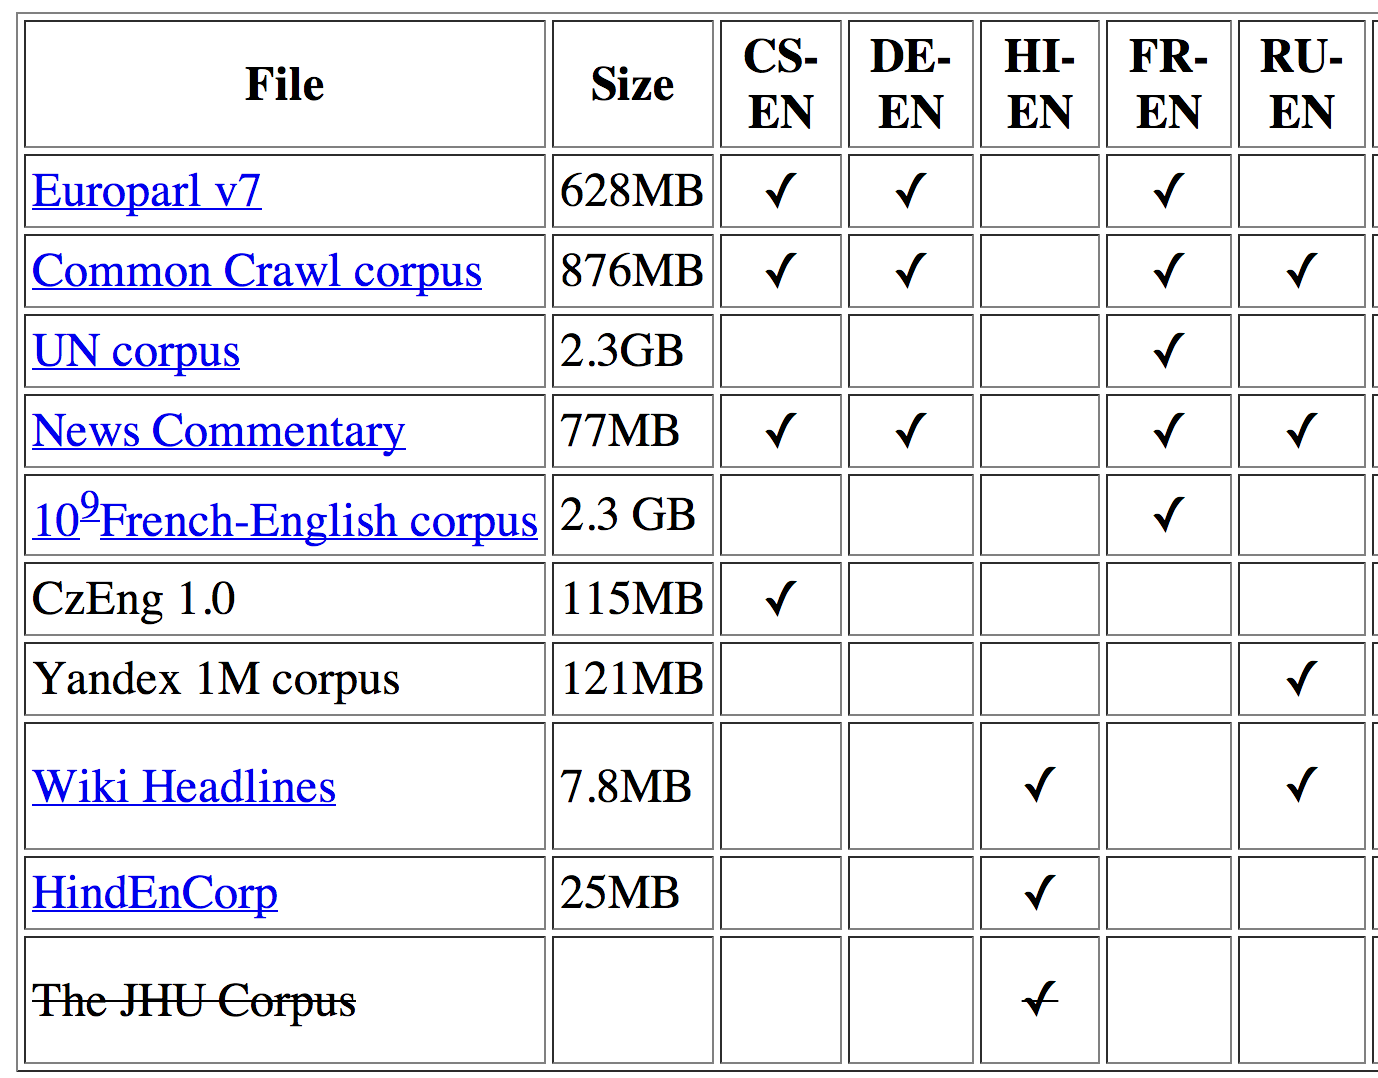
\includegraphics[scale=0.25]{wmt_data.png}
\end{center}
\caption{\scriptsize{Parallel data from WMT 2014}}
\end{figure}
\end{itemize}
\end{frame}

\begin{frame}{Motivations}
From language model (LM) perspective
\begin{itemize}
\item Recurrent neural network (RNN) can capture information about variable length sequences, which can later be decoded.
\item LMs can generate \textit{meaningful} text sequences
\begin{figure}[ht!]
\begin{center}
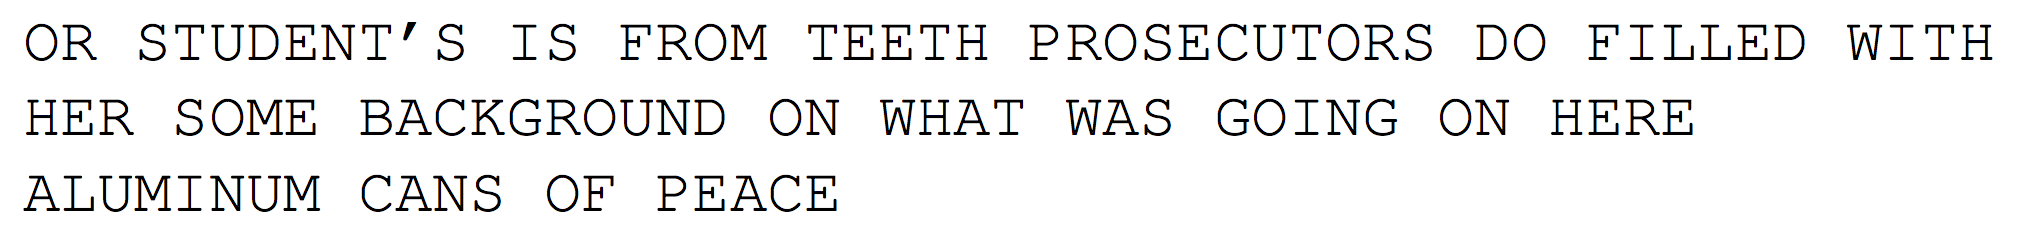
\includegraphics[scale=0.25]{4-gram.png} \\
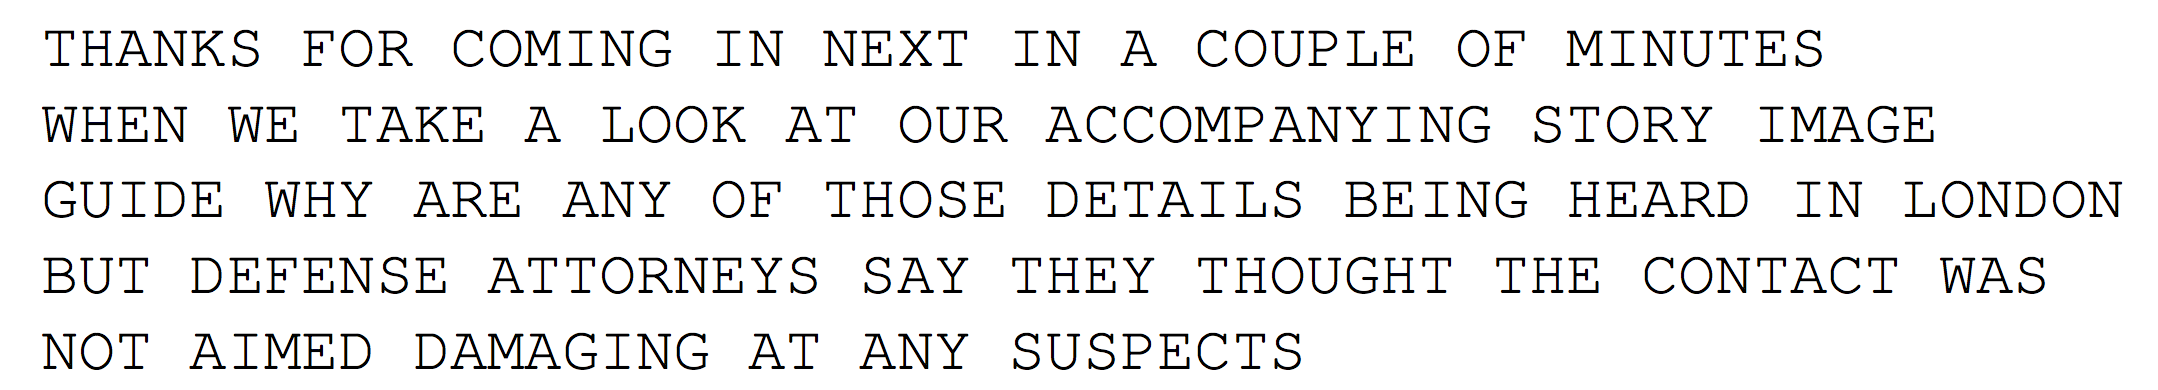
\includegraphics[scale=0.25]{rnn.png} \\
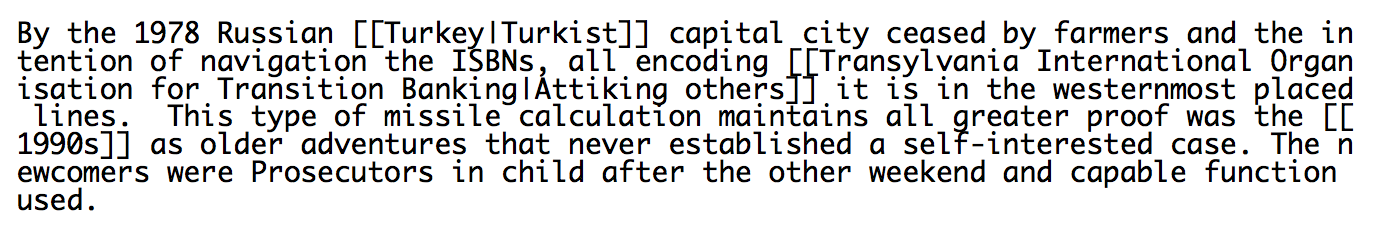
\includegraphics[scale=0.40]{rnn_char.png}
\end{center}
\caption{\scriptsize{Texts generated by some language models. Upper: 5-gram (Schwenk et al., 2007); Middle: RnnLM (Mikolov et al., 2011); Lower: Character based Deep RNN (Graves, 2014).}}
\end{figure}
\end{itemize}
\end{frame}

\begin{frame}{Recurrent neural network language model (RnnLM)}
\begin{figure}
\begin{center}
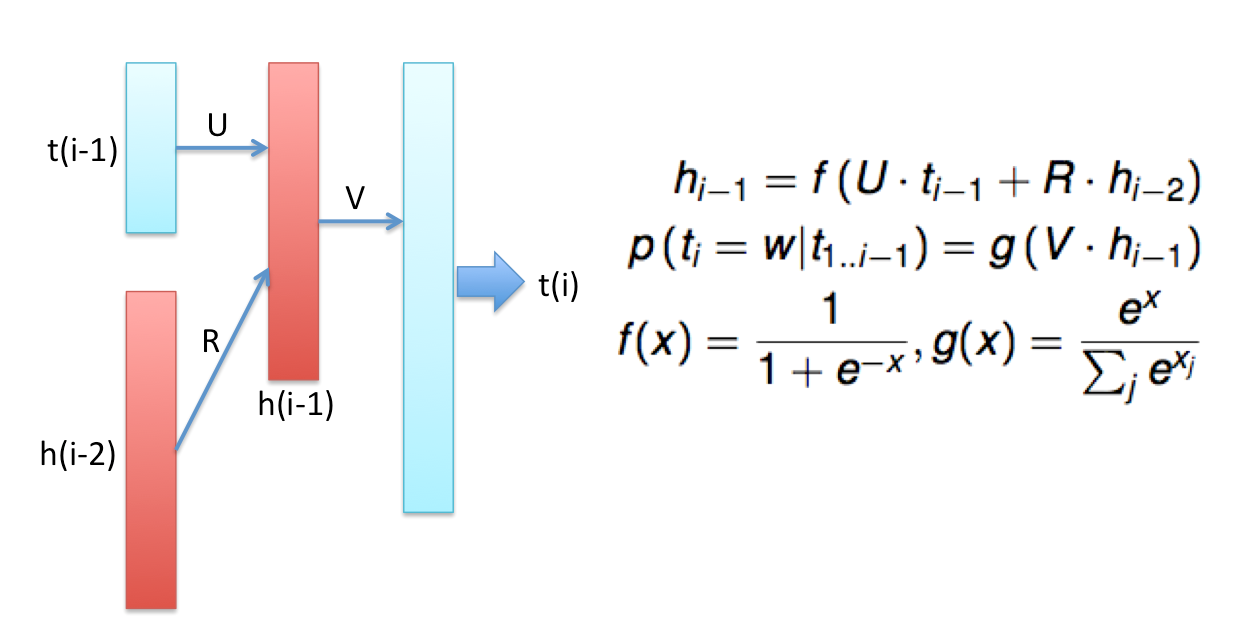
\includegraphics[scale=0.25]{rnn_standard.png}
\end{center}
\caption{Standard RnnLM (Mikolov et al., 2011)}
\end{figure}
\end{frame}
%
%\begin{frame}{Hierarchical softmax factorization}
%\begin{itemize}
%\item Why this?
%\begin{itemize}
%\item Normalization of softmax probabilities over the output is $O(\ABS{V})$ slow
%\begin{itemize}
%\item Europarl v7 (WMT '14), $\ABS{V_{En}} = 121735$, $\ABS{V_{Fr}} = 138467$.
%\item Hierarchical softmax (HS) reduces complexity to $O(\log(\ABS{V}))$.
%\end{itemize}
%\item Many words appear only once, causing difficulties estimating their embeddings.
%\end{itemize}
%\item Clustering vocab based on frequencies
%\begin{itemize}
%\item The same idea proves to work for class based RnnLM (Mikolov et al., 2011).
%\item Implementation uses weighted-balanced binary tree on vocab frequencies.
%\begin{itemize}
%\item Easy to implement, unsupervised (based on word counts from training corpora only).
%\item Frequent words are closer to the tree's root (like Huffman tree, but there is no distinct prefix constraint).
%\end{itemize}
%\end{itemize}
%\end{itemize}
%\end{frame}
%
%\begin{frame}{Hierarchical softmax factorization}
%\begin{figure}
%\begin{center}
%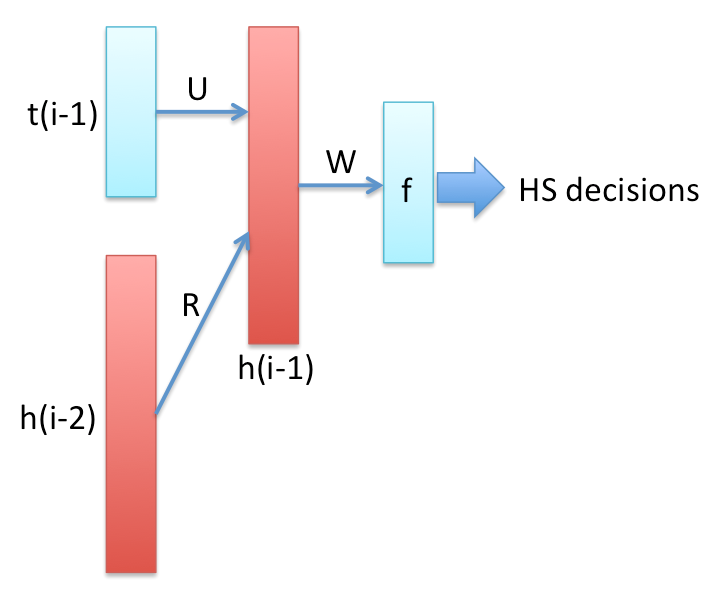
\includegraphics[scale=0.25]{rnn_hs.png}
%\end{center}
%\caption{RnnLM with HS factorization}
%\end{figure}
%\begin{itemize}
%\item Each node $p$ of the HS tree is parameterized by a vector $v_p$
%$$
%p\pc{\text{go left} | \text{at $p$}, \text{has history $t_{1..i-1}$}} = \dfrac{1}{1 + \exp{\pc{-f \cdot v_p}}}
%$$
%\end{itemize}
%\end{frame}
%
%\begin{frame}{Hierarchical softmax factorization}
%\begin{itemize}
%\item Each word $w$ is referred to as a path
%$$
%root = p_1 \to p_2 \to \cdots \to p_k = \text{a leaf}
%$$
%Probability is factored as
%$$
%p \pc{t_i = w | t_{1..i-1}} = \prod_{j = 1}^{k-1} p\pc{p_j \to p_{j+1} | p_j, t_{1..i-1}}
%$$
%\item The tree is represented by a matrix $T$, whose columns corresponds to the vectors $v_p$.
%\begin{itemize}
%\item Therefore, computing $p(t_i = w | t_{1..i-1})$ corresponds to only one column-indexed matrix multiplication.
%\item In MATLAB, this is very fast!
%\end{itemize}
%\end{itemize}
%\end{frame}
%
%\begin{frame}{Hierarchical softmax factorization}
%\begin{table}
%\begin{center}
%\begin{tabular}{| c | c | c |}
%\hline
%Hidden layer size & (Chen et al., 2014) & This work \\
%\hline \hline
%$100$ & $7.6K$ & $8.1K$ \\
%$200$ & $2.1K$ & $4.6K$ \\
%$512$ & $0.37K$ & $2.5K$ \\
%$800$ & $0.11K$ & $1.8K$ \\
%\hline
%\end{tabular}
%\caption{\scriptsize{Comparison of words trained per second with (Chen et al., 2014), which uses GPU-based and sentence bunch mode. We only train on single thread CPU, with minibatch size of $500$.}}
%\end{center}
%\end{table}
%\end{frame}

%\begin{frame}{Joint bilingual RnnLM}
%\begin{figure}
%\begin{center}
%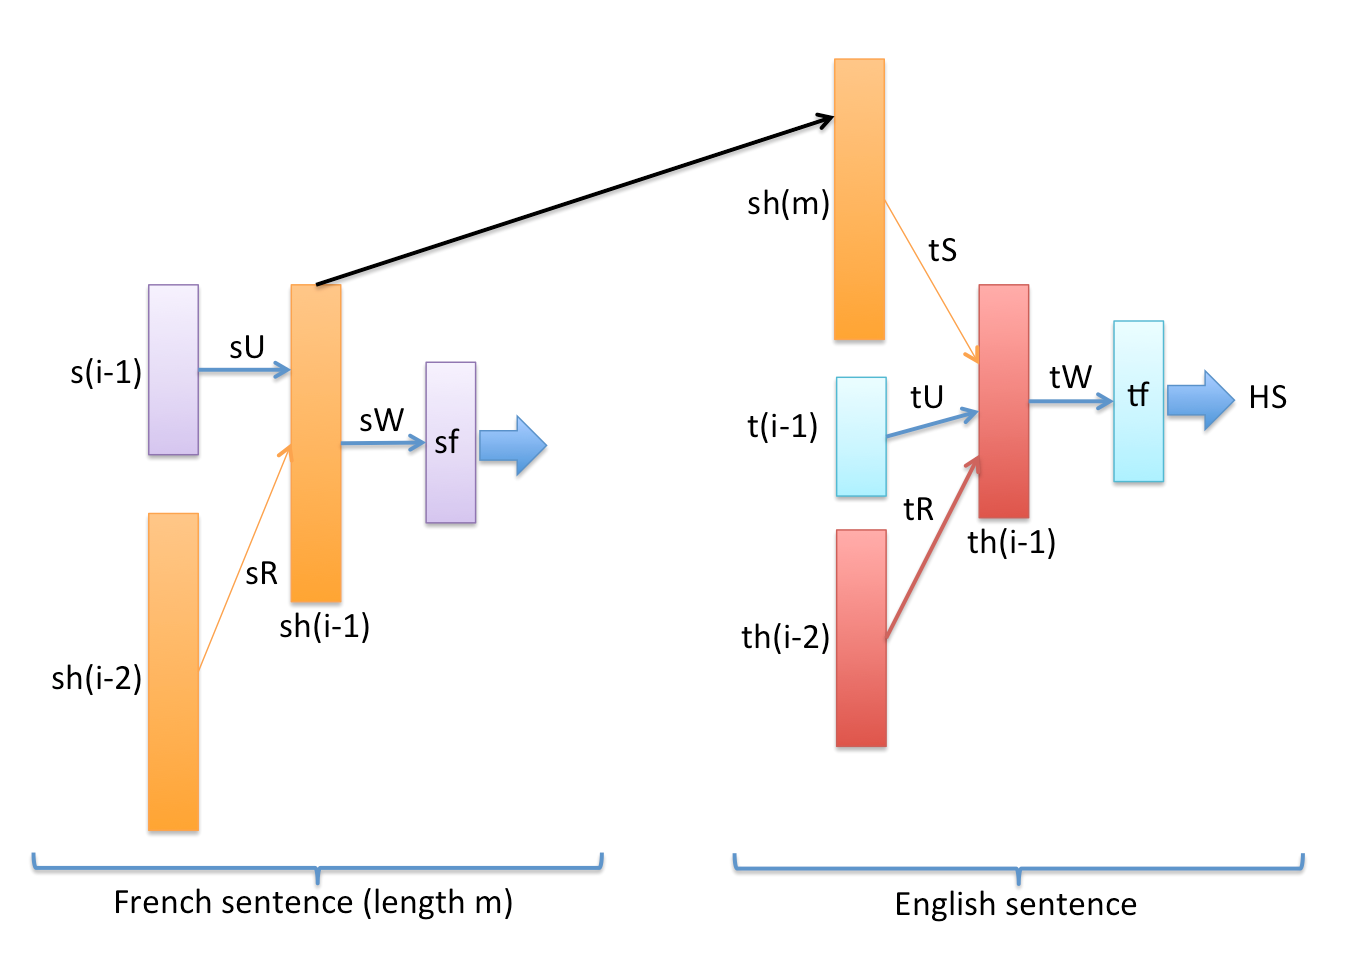
\includegraphics[scale=0.22]{pipe_rnn.png}
%\end{center}
%\caption{Architecture of joint bilingual RnnLM}
%\end{figure}
%\end{frame}

\begin{frame}{Joint bilingual RnnLM}
\begin{figure}
\begin{center}
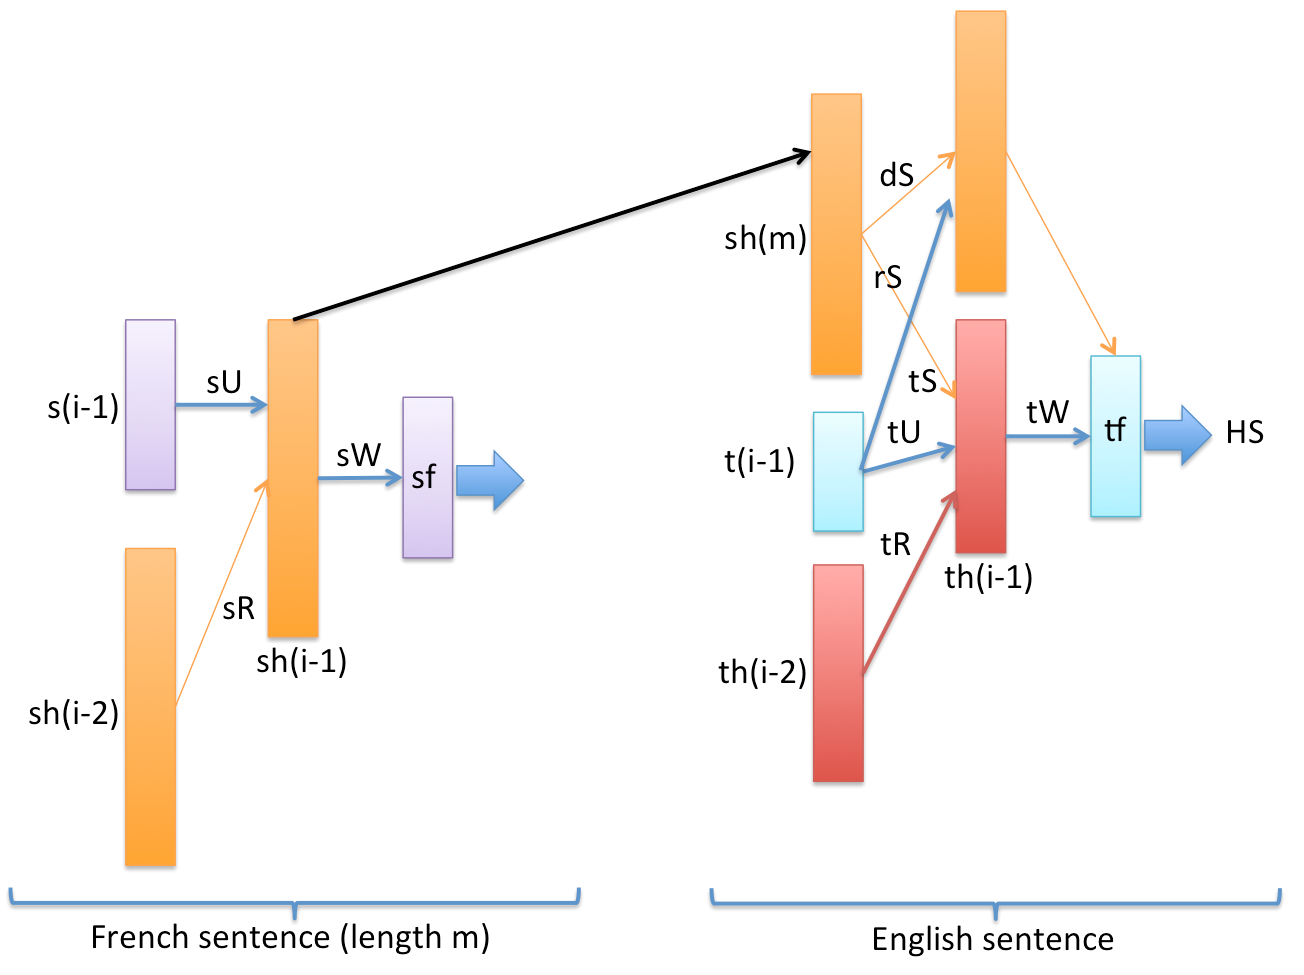
\includegraphics[scale=0.225]{unroll_pipe_rnn.png}
\end{center}
\caption{\scriptsize{Architecture of source unrolled joint bilingual RnnLM.}}
\end{figure}
\end{frame}

\begin{frame}{Joint bilingual RnnLM}
\begin{itemize}
\item Source (fr): $s_1 s_2 \cdots s_m$; target (en): $t_1 t_2 \cdots t_n$
\item Hypotheses:
\begin{itemize}
\item The hidden layer of RnnLM can capture important semantics meaning of partial histories of the sentence
\begin{itemize}
\item Thus the final values of the hidden layer capture the whole sentence's meaning.
\end{itemize}
\item These information can be ``retrieved''
\end{itemize}
\item We use the ``meaning'' of the source to bias the RnnLM of the target
\begin{align*}
&tgtH_{i-1} = f \pc{U \cdot t_{i-1} + R \cdot tgtH_{i-2}} \\
\text{ becomes } &tgtH_{i-1} = f \pc{U \cdot t_{i-1} + R \cdot h_{i-2} + S \cdot srcH(m)}
\end{align*}
\item This can be extended further to ``guide'' the target model to ``unroll'' $srcH(m)$ and retrieve its meaning.
\end{itemize}
\end{frame}

%\begin{frame}{Source unrolled joint bilingual RnnLM}
%\begin{itemize}
%\item At each time step, we update the bias on the target RNN by
%\begin{align*}
%srcH_{0} &= \text{final representation of source sentence} \\
%srcH_{i-1} &= f \pc{dS \cdot srcH_{i-2} + rS \cdot t_{i-1}}
%\end{align*}
%\end{itemize}
%\end{frame}

\begin{frame}{Experiments}
\begin{itemize}
\item Data: Europarl v7 fr-en, WMT '14
\begin{itemize}
\item $2.2M$ parallel sentences, leaving out $20K$ sentences for validation.
\item Vocab sizes: $\ABS{V_{En}} = 121735$, $\ABS{V_{Fr}} = 138467$.
\end{itemize}
\item Training is done via stochastic gradient descent
\begin{itemize}
\item Minimize sum of cross entropy errors at each word in both source and target sentences.
\item 7 epochs with learning rate decaying after each epoch.
\item Gradient is computed via the traditional backprogation through time (BPTT) algorithm.
\begin{itemize}
\item We did not truncate BPTT, nor did we clip the gradient to lower than some value.
\item We observed no gradient explosion as reported and cautioned in (Mikolov et al., 2011), (Le et al., 2010).
\end{itemize}
\end{itemize}
\item The learned model are then used to generate ``translations'' via a beam decoder for best target sequences (not yet...)
\end{itemize}
\end{frame}

\begin{frame}{Results}
\begin{itemize}
\item Perplexities
\begin{figure}
\begin{center}
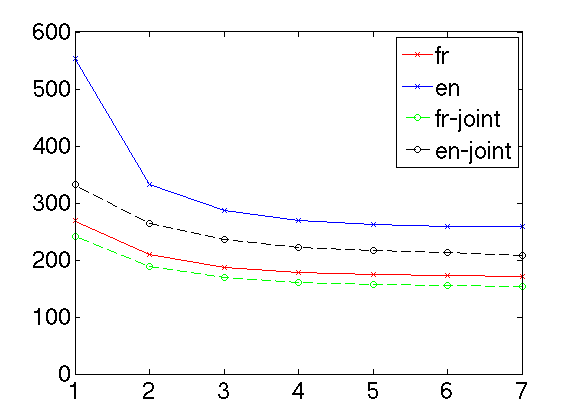
\includegraphics[scale=0.35]{ppl.png}
\end{center}
\caption{\scriptsize{Perplexities on joint model are smaller than those on independent models.}}
\end{figure}
\end{itemize}
\end{frame}

\begin{frame}{Results}
\begin{itemize}
\item Lexical translation
\begin{itemize}
\item Given a French word $f$, we encode it using the RNN model on source side, then compute the probabilistic distribution over the words in target dictionary.
\item Translated words are compared against the first word translated by Google Translator.
\item Result: $81.3 \%$ lexical translations match!
\begin{itemize}
\item We have (nearly) inferred the dictionary!
\end{itemize}
\item Some wrong translations
\begin{table}
\begin{center}
\begin{tabular}{| c | c | c |}
\hline
French & English gold & English translated \\
\hline \hline
legalement & legally & legal \\
meme & same & , (comma) \\
exactement & exactly & right \\
connaître & know & taste \\
confidentialité & confidentiality & <unk> \\
\hline
\end{tabular}
\end{center}
\end{table}
\end{itemize}
\end{itemize}
\end{frame}

\begin{frame}
\begin{figure}
\begin{center}

\includegraphics[scale=0.9]{thankyou.jpg}
\end{center}
\end{figure}
\end{frame}
\end{document}